\chapter{Expectation-maximization applied to brain segmentation}\label{sec:EM}
%Each main chapter or section should start with a short description of
%what it holds, and why. Top tip --- begin the whole writing enterprise
%with a first draft of this little bit for each chapter. It will force
%you to think about overall structure.\\get
%dsfdfs
%\par
%
Here we get going with theory of the expectation-maximization (EM) applied to brain segmentation. We show firstly a simple approach of the problem, in the particular case of Gaussian Mixture Models (GMM) followed by a more generalistic approach. The simple approach will give you an intuitive understanding of the problem then the general approach will formalize it in order to adapt it to most of the segmentation problems. Finally, there will be a presentation of the algorithm used in Slicer 3\footnote{open source software developped in the SPL for biomedical engineering purpose}.
%
\section{Presentation of the EM segmentation}
%Magnetic resonance imaging (MRI) is very well suited for analyzing human soft tissue anatomy. It provides high resolution high resolution 3D volumetric data with high resolution between soft tissues. Nevertheless, this technique has some disavantages. Indeed MRI images can be alterated by some artifacts as movement, magnetic suceptibility, http://www.e-mri.org, aliasing, etc.. Another main problem is the apparition of a bias on MRIs. This bias results from QDSFQSDF. Correcting this problem is very important in the purpose of image processing. If we don't, the same tissue will have different intensities through the volume, which can bree mistakes during the segmentation process.
The EM algorithm was originally described in 1977 by Arthur Dempster, Nan Laird, and Donald Rubin\cite{1}. They generalized and developped a method used in several times by authors, for particular applications. It is widely used to solve problems where data are "missing". %In our particular purpose of brain segmentation, the missing data is the knowledge of the tissues.
The EM algorithm is an iterative algorithm which works in two steps: Expectation and Maximization. It can be use to solve a lot of image processing's problems like classification, restoration\cite{3}, motion estimation\cite{2}, etc.. 
Since the generalization of the algorithm, a lot of related papers were proposed. Most of them bring algorithms derived from the original one to adapt it to particuliar problems using additional informations like spatial or structural information.
\par
Nowadays, EM algorithms are become a popular tool for classification problems.  It is particulary well suited for brain MR images segmentation.
A lot of algorithms already exist. They present complex frameworks using spatial information, neighborhood or intensity inhomogeneities to enhance the classification.\\
In the SPL, the algorithm developped uses spatial, structural and intensity inhomogeneities informations to segment the brain. 
%

\section{Fundamentals}
%
Here we get going with a presentation of all the fundamentals you need to have a good understanding of EM segmentation. We begin with a description of the statistical model used for the brain. Then we present briefly the widely used GMM. Finally we will introduce you to what the mamixum likelihood function. This part is mainly inspired from \cite{4}, \cite{5} and \cite{6}
%
\subsection{Statistical model used for the brain}
%
We define the voxel intensities of a MR image as $Y=\lbrace y_1, ..., y_n\rbrace$ when the image consisted in $n$ voxels. Each $y$ intensity is called \textit{observed data} because this is the the data we see when we observe the image. Each $y$ is a realization of the random variable $Y$. The real labelling of the image is $Z$. $Z$ is called \textit{hidden data} because we don't know the value of each label. This is precisely the purpose of the segmentation: estimating the \textit{hidden data} from the \textit{observed data}. We assume that the \textit{observed data} is generated from the \textit{hidden data} and a parameter $\Phi$. The parameter $\Phi$ can either be a probability density function, noise, bias field, etc., depending on the model.
\par
$Y$ and $Z$ can be viewed as $n$-dimensional random variables $Y=\lbrace Y_1, ..., Y_n\rbrace$ and $Z=\lbrace Z_1, ..., Z_n\rbrace$ then each $y_i$ is a realisation of $Y_i$ and each $z_i$ is a realization of $Z_i$.The conditional probability function describing $Y_i$ is $p(Y_i|Z_i,\Phi)$.
\par
The easiest model assumes that each intensity in one class is the same, but this intensity is corrupted by factors like noise,  with a Gaussian Distribution. We can describe the relationship as below:
  
  \begin{equation*}
  y_i=\mu_k+n_i\\
  \end{equation*}

\par
where $\mu_k$ is the mean intensity of the $k^th$ tissue and $n_i$ a random sample generated by the corrupting factor(s). Let's say that $n_i$ is generated by a Gaussian probability distribution function $G(.,0,\sigma)$, with $0$ mean and $\sigma$ variance. That means that $y_i$ is a random sample generated by Gaussian probability density function $G(.,\mu_k,\sigma)$. Let's assume that each class has a different variance, $G(.,\mu_k,\sigma)$ becomes $G(.,\mu_k,\sigma_k)$ and it leads to:
  
  \begin{equation}\label{CDP}
  p(Y_i=y_i|Z_i=k,\Phi)=G(y_i,\mu_k,\sigma_k)\\
  \end{equation}

\par
As the labelling is not known, it is usefull to express the probability density function (PDF) of $Y_i$ only depending on parameter $\Phi$ with the total probability theorem:

  \begin{equation}\label{PDF}
  p(Y_i|\Phi)=\sum_{k=1}^K p(Y_i=y_i|Z_i=k,\Phi)p(Z_i=k|\Phi)\\
  \end{equation}

\par
$p(Z_i=k|\Phi)$ is the \textit{prior probability}. It expresses the probability that a voxel $i$ belongs to a class $k$. $p(Y_i=y|Z_i=k,\Phi)$ is the \textit{likelihood}. In our case, we will assume that the \textit{prior probability} is constant. The new model we obtain for the labelling, via a gaussian distribution,  is a widely used one: the \textit{Gaussian mixture model}.
%
\subsection{Gaussian mixture model}
Let's remind the first hypotesis: the conditional probability function for each tissue to segment is Gaussian equation ~(\ref{CDP}). Moreover, we will assume that \textit{prior probability} is a constant $c_k$ for each class $k$. $c_k$ is the \textit{weight} of the class $k$.
  
  \begin{equation}\label{CW}
  p(Z_i=k|\Phi)=c_k\\
  \end{equation}

The last assumption will be that $\Phi$ contains unknown means, variances and weights for each tissue. Then we can express $\Phi$ as $\Phi=(\mu_1, \sigma_1, c_1, ..., \mu_K, \sigma_K, c_K)$.
\par
Using equations ~(\ref{CDP}) and (\ref{CW}), equation ~(\ref{PDF}) becomes:
 
  \begin{equation}\label{GMM}
  p(Y_i=y|\Phi)=\sum_{k=1}^K G(y,\mu_k,\sigma_k)c_k\\
  \end{equation}

\par
In the case of \textit{Gaussian mixture model}, each voxel is considered to be independent. That means that each voxel will have his own probability density function. Consequently, the normalized histogram of the whole volume can be interpreted as an approxmation of the sum of all the probability density functions. %The next step is then to find the set $(\mu_i, \sigma_i, c_i)$ of parameter $\Phi$  for each voxel, to fit as well as possible the normalized histogram. A convenient way to find it is to use the \textit{Maximum likelihood} principle.
%
\subsection{Maximum likelihood}
In our case, we know the intensity of each observed pixel $y_i$. $\Phi$ has to be found. The best estimation of $\Phi$ will be obtain using the maximum likelihood principle. $p(Y=y_i|\Phi)$ is called likellihood function and for it returns the value of the likelihood for $y_i$, given $\Phi$. We can generalize it to the whole image with $p(Y|\Phi)$.
\par
The voxels are considered to be independent through the whole volume. It leads us to:
 
  \begin{equation}\label{ML}
  p(Y|\Phi)= \prod_{i=1}^n p(Y_i|\Phi)\\
  \end{equation}

\par
We must keep in mind that the objective is to find the parameter $\Phi$ which will maximize the likelihood of the observed volume. We can note this parameter:
  
  \begin{equation}\label{AR}
  \hat{\Phi}=\operatorname*{arg\,max}_\Phi p(Y|\Phi)\\
  \end{equation}

\par
Therefore, it is more convenient to work with logarithm because the product from equation ~(\ref{ML}) will be converted into a sum. Equation ~(\ref{AR}) becomes:
  
  \begin{equation*}\label{ARL}
  \hat{\Phi}=\operatorname*{arg\,max}_\Phi \operatorname*{log} p(Y|\Phi). %=\operatorname*{arg\,max}_\Phi L(\Phi)\\
  \end{equation*}

Let us denote:

  \begin{align*}
  L(\Phi) &\triangleq \operatorname*{log} p(Y|\Phi) \\
          &= \sum_{i=1}^n \operatorname*{log}\sum_{k=1}^K p(Y_i=y|Z_i=k,\Phi)p(Z_i=k|\Phi)\\
  \end{align*} 

Finally, in case of GMM, with eq.~(\ref{GMM}), $L(\Phi)$ becomes:
  
  \begin{equation*}\label{LP}
  L(\Phi)=\sum_{i=1}^n \operatorname*{log} \sum_{k=1}^K G(y,\mu_k,\sigma_k)c_k\\
  \end{equation*}

The maximized $log$ likelihood can then be computed using partial derivatives for each paraemter of $\Phi$. When the partial derivative of $L(\Phi)$ is $0$ for a parameter, we found the maximum likelihood for the parameter.
\par
For example, to find the maximum likelihood for $\mu_k$, we have to find when:

  \begin{equation*}\label{PD}
  \frac{\partial}{\partial\mu_k}(L(\Phi))=0\\
  \end{equation*}

\par
Then we compute the partial derivative of $L(\Phi)$ over $\mu_k$:
%\begin{equation}\label{PDF}

  \begin{align}\label{partialDerivative}
  \frac{\partial}{\partial\mu_k}(L(\Phi)) &= \frac{\partial}{\partial\mu_k}( \sum_{i=1}^n \operatorname*{log} \sum_{k=1}^K G(y,\mu_k,\sigma_k)c_k\nonumber)  \\
                                          &= \sum_{i=1}^n \frac{G(y,\mu_k,\sigma_k)c_k}{\sum_{j=1}^K G(y,\mu_j,\sigma_j)c_j}\frac{\partial}{\partial\mu_k}  (-\frac{(y-\mu_k)^2}{2\sigma_k^2}) \nonumber \\
                                          &= \sum_{i=1}^n \frac{G(y,\mu_k,\sigma_k)c_k}{\sum_{j=1}^K G(y,\mu_j,\sigma_j)c_j}(\frac{(y-\mu_k)}{\sigma_k^2}) \nonumber \\
                                          &= \sum_{i=1}^n \frac{p(Y_i=y|Z_i=k,\Phi)p(Z_i=k|\Phi)}{\sum_{j=1}^K p(Y_i=y|Z_i=j,\Phi)p(Z_i=j|\Phi)}(\frac{(y-\mu_k)} {\sigma_k^2})
  \end{align}

%\end{equation}
%Let's introduce the \textit{posterior probability}. It expresses the probability that a voxel belongs to a tissue. It is also called \textit{soft assignement} of %\textit{soft segmentation}. The probability that a pixel $i$ belongs to a class $j$ is:
% \begin{equation}\label{PP}
%  p(Z_i=j|Y_i=y_i,\Phi)
%  \end{equation}
Using Bayes' theorem (see App.~\ref{app:formulas}, Sec.~\ref{f:Bayes}), we notice that:

  \begin{equation}\label{BF}
  p(Z_i=k|Y_i=y_i,\Phi)= \frac{p(Y_i=y_i|Z_i=k,\Phi)p(Z_i=k|\Phi)}{\sum_{j=1} p(Y_i=y_i|Z_i=j,\Phi)p(Z_i=j|\Phi)}\\
  \end{equation}

Thus, setting the denominator to 0 in equation ~(\ref{partialDerivative}) and using equation ~(\ref{BF})yields:
 
  \begin{equation}\label{YY}
  \sum_{i=1}^n p(Z_i=k|Y_i=y_i,\Phi)(y-\mu_k)=0\\
  \end{equation}

%The \textit{posterior probability} helps us to define the \textit{probability map}.
Let us denote

  \begin{equation}%\label{}
  p_{ik}=p(Z_i=k|Y_i=y_i,\Phi)\\
  \end{equation}

Equation ~(\ref{YY}) leads us to:
 
  \begin{equation}\label{MU}
  \mu_k = \frac{\sum_{i=1}^n y_ip_{ik}}{\sum_{i=1}^n p_{ik}}\\
  \end{equation}
Proceeding the same way as we did for equation ~(\ref{YY}), we can get similar equations for variance $\sigma_j$ and weight $c_j$. 

We find that:

  \begin{equation}\label{SI}
  \sigma_k^2 = \frac{\sum_{i=1}^n (y_i-\mu_k)^2p_{ik}}{\sum_{i=1}^n p_{ik}}\\
  \end{equation}
  
  \begin{equation}\label{WE}
  c_k = \frac{1}{n}\sum_{i=1}^n p_{ik}\\
  \end{equation}

\par
Equations ~(\ref{MU}),(\ref{SI}), and (\ref{WE}) provides us an equation for soft segmentation. This equation expresses that a voxel $i$ belongs to the class $k$.
  
  \begin{equation}\label{SS}
  p_{ik}= \frac{G(y_i,\mu_k,\sigma_k)c_k}{\sum_{j=1}^K G(y_i,\mu_j,\sigma_j)c_j}\\
  \end{equation}

In the case og GMM, the segmentation can now be done following an iterative algorithm called \textit{expectation maximization algorithm}.
%
\section{Expectation maximization algorithm}
The EM algorithm is a method to find the maximum likelihood for a given set of parameter ($\Phi$ in our case). Here we first get going with an 
intuitive description of the algorithm in the particular case of GMM then we will present a more general definition.
%
\subsubsection{Algorithm in case of Gaussian mixture data model}
Let's assume that we can find the maximum likelihood of the hidden data by a direct differentiation (because of the GMM). The EM algorithm is an iterative process of two steps: the expectation step (E-Step) and the maximization step (M-Step). At each iteration, the maximum likelihood will be increased until convergence is reached.\\
\begin{itemize}

\item \textbf{E-step}\\
In this step, we calculate an estimation of soft segmentation $p^{(m+1)}$ with equation ~(\ref{SS}) as below. We know all the variables needed for the calculation from the observed data and the current parameter estimate $\Phi^{(m)}$. Note that an initialization is necessary for the first iteration.\\

  \begin{equation*}
  p_{ik}^{(m+1)}= \frac{G(y_i,\mu_k^{(m)},\sigma_k^{(m)})c_k^{(m)}}{\sum_{j=1}^K G(y_i,\mu_j^{(m)},\sigma_j^{(m)})c_j^{(m)}}\\
  \end{equation*}

\item \textbf{M-step}\\
In this step, we estimate the maximum likelihood for parameter $\Phi^{(m+1)}$. We do it with equations ~(\ref{MU}),(\ref{SI}), and (\ref{WE}) as below. We know all the variables needed for the calculation from the observed data and the current estimate $p^{(m+1)}$ of hidden data.\\

  \begin{equation*}
  \mu_k^{(m+1)} = \frac{\sum_{i=1}^n y_ip_{ik}^{(m+1)}}{\sum_{i=1}^n p_{ik}^{(m+1)}}\\
  \end{equation*}

  \begin{equation*}
  (\sigma_k^{(m+1)})^2 = \frac{\sum_{i=1}^n (y_i-\mu_k^{(m+1)})^2p_{ik}^{(m+1)}}{\sum_{i=1}^n p_{ik}^{(m+1)}}\\
  \end{equation*}
  
  \begin{equation*}
  c_k^{(m+1)} = \frac{1}{n}\sum_{i=1}^n p_{ik}^{(m+1)}\\
  \end{equation*}
\end{itemize}

%EM algorithm iterates until convergence is reached. 
%As discussed in \cite{7} , convergence is assured since the algorithm is guaranted to increase the likelihood at each iteration.
The problem is simple as long as we are working with GMM. In the other case, the log-likelihood can not be maximized by direct differenciation and a more generalized approach must be used.
%
\subsubsection{Generalized algorithm}\label{GENERAL}
Now we assume that we are no longer working with GMM. Thus, we must use a more general algorithm. %We will first present briefly the E-Step and the M-Step. Then we will explain the function used in both steps and finally we will show how we can use it for the specific problem of segmentation.\\
To explain the general algorithm, we will start from the log-likelihood $L(\Phi)$. As presented in the previous subsection:

  \begin{equation*}
  L(\Phi)=\operatorname*{log} p(Y|\Phi)\\
  \end{equation*}
 
Since $log$ is a strictely increasing function, the value of $\Phi$ which will maximizes  $p(Y|\Phi)$ will also maximizes $L(\Phi)$. We want to maximize $L(\Phi)$. Thus, after the $m^{th}$ iteration, we want an estimated $\Phi_n$ such as:

  \begin{equation*}
  L(\Phi)>L(\Phi^{(m)})
  \end{equation*}
 
In other words, we want to maximize the difference $L(\Phi)-L(\Phi_n)$. For convenience, we introduce a new variable $z_{ik}$ which means that $Z_i=k$. Using the new notation, we can transform this difference as below:

 
  \begin{align*}
  L(\Phi)-L(\Phi_n) &=\operatorname*{log} p(Y|\Phi) -\operatorname*{log} p(Y|\Phi_n)\\
                    &=\sum_{i=1}^n\{\operatorname*{log} \sum_{k=1}^K p(Y_i|z_{ik},\Phi)p(z_{ik}|\Phi)-\operatorname*{log} p(Y_i|\Phi_n)\}\\
                    &=\sum_{i=1}^n\{\operatorname*{log} \sum_{k=1}^K p(Y_i|z_{ik},\Phi)p(z_{ik}|\Phi).\frac{p(z_{ik}|Y_i,\Phi_n)}{p(z_{ik}|Y_i,\Phi_n)}-\operatorname*{log} p(Y_i|\Phi_n)\}\\
                    &=\sum_{i=1}^n\{\operatorname*{log} \sum_{k=1}^K p(z_{ik}|Y_i,\Phi_n).\frac{p(Y_i|z_{ik},\Phi)p(z_{ik}|\Phi)}{p(z_{ik}|Y_i,\Phi_n)}-\operatorname*{log} p(Y_i|\Phi_n)\}\\
                    &\geq \sum_{i=1}^n\{\sum_{k=1}^K p(z_{ik}|Y_i,\Phi_n)\operatorname*{log} \frac{p(Y_i|z_{ik},\Phi)p(z_{ik}|\Phi)}{p(z_{ik}|Y_i,\Phi_n)}-\operatorname*{log} p(Y_i|\Phi_n)\}
  \end{align*}

We can deduce this inequality from Jensen's inequality (see App.~\ref{app:formulas}, Sec.~\ref{f:Jensen}) since  $p(z_{ik}|Y_i,\Phi^{(m)})$ is a probability mesure and $ln$ a concave function (\cite{5}). %Indeed, 

%  \begin{equation*}
%  p(z_{ik}|Y_i,\Phi_n)>0\\
%  \end{equation*}
%  \begin{equation*}
%  \sum_k p(z_{ik}|Y_i,\Phi_n)=1\\
%  \end{equation*}
\par
We will then use the fact that  $\sum_k p(z_{ik}|Y_i,\Phi^{(m)})=1$. In this case, it leads to $\operatorname*{log} p(Y|\Phi^{(m)})=\sum_k p(z_{ik}|Y_i,\Phi^{(m)})\operatorname*{log} p(Y|\Phi^{(m)})$. This allows us to bring $\operatorname*{log} p(Y|\Phi^{(m)})$ into the summation. 
\par
We will also use a new variable $e_k$ to express the difference through the whole volume without a summation. $e_k$ is defined as $e_k=\{z_{1k}, ..., z_{nk}\}$ when the image consisted in $n$ voxels. For example, $z_{ik}=e_k=\{0,...,0,1,0,...,0\}$ means that voxel $i$ belongs to class $k$.

  \begin{align*}
  L(\Phi)-L(\Phi_n) &\geq \sum_{i=1}^n\{\sum_{k=1}^K p(z_{ik}|Y_i,\Phi^{(m)})\operatorname*{log} \frac{p(Y_i|z_{ik},\Phi)p(z_{ik}\Phi)}{p(z_{ik}|Y_i,\Phi^{(m)})}-\operatorname*{log} p(Y|\Phi^{(m)})\} \\
                    &=\sum_{i=1}^n\{\sum_{k=1}^K   p(z_{ik}|Y_i,\Phi^{(m)})\operatorname*{log} \frac{p(Y_i|z_{ik},\Phi)p(z_{ik}|\Phi)}{p(z_{ik}|Y_i,\Phi^{(m)})p(Y_i|\Phi^{(m)})}\}\\
                    &=\sum_{k=1}^K   p(e_{k}|Y,\Phi^{(m)})\operatorname*{log} \frac{p(Y|e_{k},\Phi)p(e_{k}|\Phi)}{p(e_{k}|Y,\Phi^{(m)})p(Y|\Phi^{(m)})}\\
                    &\triangleq \Delta(\Phi|\Phi_n
  \end{align*}

We can then conclude that:

  \begin{align*}
  L(\Phi) &\geq L(\Phi^{(m)}) + \Delta(\Phi|\Phi^{(m)})\\
          &\geq l(\Phi|\Phi^{(m)})
  \end{align*}

where $l(\Phi|\Phi^{(m)}) \triangleq  L(\Phi{(m)}) + \Delta(\Phi|\Phi^{(m)})$.\\
\par
We have now a function $l(\Phi|\Phi^{(m)})$ which is bounded above by $L(\Phi)$. The only time when the two functions are egals is when $\Phi=\Phi^{(m)}$.
Our objective is to find the value of $\Phi$ which will maximize $L(\Phi)$. \\
%From equation ~(\ref{ineq}), we deduce that each $\Phi$ which increases $l(\Phi|\Phi_n)$ will increase $L(\Phi)$ too.
We can formalize this research. $\Phi^{(m+1)}$ is the updated value which is get after maximization of $\Phi$ using $\Phi^{(m)}$. %Once $\Phi^{(m)}=\Phi^{(m+1)}$, the algorithm has converged.

  \begin{align}\label{eMF}
  \Phi^{(m+1)} &= \operatorname*{arg\,max}_\Phi \{l(\Phi|\Phi^{(m)})\} \nonumber \\         
             &= \operatorname*{arg\,max}_\Phi \{L(\Phi^{(m)}) + \sum_{k=1}^K   p(e_{k}|Y,\Phi^{(m)})\operatorname*{log} \frac{p(Y|e_{k},\Phi)p(e_{k}|\Phi)}{p(e_{k}|Y,\Phi^{(m)})p(Y|\Phi^{(m)})}\} \nonumber \\
             &\mbox{As $p(e_{k}|Y,\Phi^{(m)})$ and $p(Y|\Phi^{(m)})$ do not depend on $\Phi$} \nonumber \\
             %&{now we remove the terms which are constants regarding \Phi }\\
             &=\operatorname*{arg\,max}_\Phi \{\sum_{k=1}^K   p(e_{k}|Y_i,\Phi^{(m)})\operatorname*{log} p(Y|e_{k},\Phi)p(e_{k}|\Phi) \} \nonumber \\
             &=\operatorname*{arg\,max}_\Phi \{\sum_{k=1}^K   p(e_{k}|Y,\Phi^{(m)})\operatorname*{log} \frac{p(Y,e_{k},\Phi)p(e_{k},\Phi)}{p(e_{k},\Phi)p(\Phi)}\}      \nonumber \\
             &=\operatorname*{arg\,max}_\Phi \{\sum_{k=1}^K   p(e_{k}|Y,\Phi^{(m)})\operatorname*{log} p(Y,e_{k}|\Phi)\} \\
             &=\operatorname*{arg\,max}_\Phi \{ E_{Z|Y,\Phi^{(m)}} \{\operatorname*{log} p(Y,Z|\Phi)\}\} \nonumber
  \end{align}
  
We notice from equation ~(\ref{eMF}), that , for a given voxel $i$:

  \begin{equation}\label{BAYES}
  \sum_{k=1}^K   p(e_{k}|Y_i,\Phi^{(m)})\operatorname*{log} p(Y_i,e_{k}|\Phi) = \sum_{k=1}^K   p_{ik}^{(m+1)}\operatorname*{log} p(Y_i,e_{k}|\Phi)
  \end{equation}

Now, both expectation and maximization steps are apparents.\\
\begin{itemize}
\item \textbf{E-step}\\
This this the expectation step. During this step, we estimate the probability that the pixel $i$ belongs to class $k$ regarding $\Phi_{(m)}$. This equation is obtained from equation ~(\ref{BAYES}) with Bayes formula.

  \begin{equation}\label{ESTEP1}
  p_{ik}^{(m+1)} = \frac{p(Y_i|e_k,\Phi^{(m)})p(e_k|\Phi^{(m)})}{\sum_{j=1}^K   p(Y_i|e_j,\Phi^{(m)}) p(e_{j}|\Phi^{(m)})}  
  \end{equation}
$p_{ik}$ is used to fill a "map" of soft segmentation. At the end of the segmentation, This map contains the probability that the voxel $i$ belongs to class $1, 2, ..., K$. We determine the class of the pixel $i$ looking at the class which has the highest probability for this given voxel $i$.
Using this probability, $E_{Z|Y,\Phi^{(m)}}$ returns the expected value of the parameter $\Phi$ regarding $\Phi^{(m)}$.\\


\item \textbf{M-step}\\
This this the maximization step. During this step $\operatorname*{arg\,max}_\Phi$ maximizes $E_{Z|Y,\Phi^{(m)}}$ for the parameter $\Phi$. It returns $\Phi^{(m+1)}$
  \begin{equation}
  \operatorname*{arg\,max}_\Phi \{ E_{Z|Y,\Phi^{(m)}} \{\operatorname*{log} p(Y,Z|\Phi)\}\}\\
  \end{equation}
 
\end{itemize} 
  
The EM algorithm iterates until convergence is reached. The condition of convergence can differ from an algorithm to another. A possibility is to fix the number of iterations of the algorithm. Most of the time, the following approach is used; convergence is reached when the difference between the estimation of the parameter $\Phi$, at step $m$ and step $m+1$ is smaller than $\varepsilon$:

  \begin{equation*}
  \Phi^{(m+1)}-\Phi^{(m)} < \varepsilon
  \end{equation*}

If after the $C^{th}$ iteration, this condition is not satisfied, the EM algorithm is stopped. \\

 
  \par
  We are now familiar with the theory behind the EM algorithm. The logic appears clearly and we can summarize the basic algorithm with the figure ~(\ref{fig:EMAlgorithm}):
   
  \begin{figure}[ht]\centering
  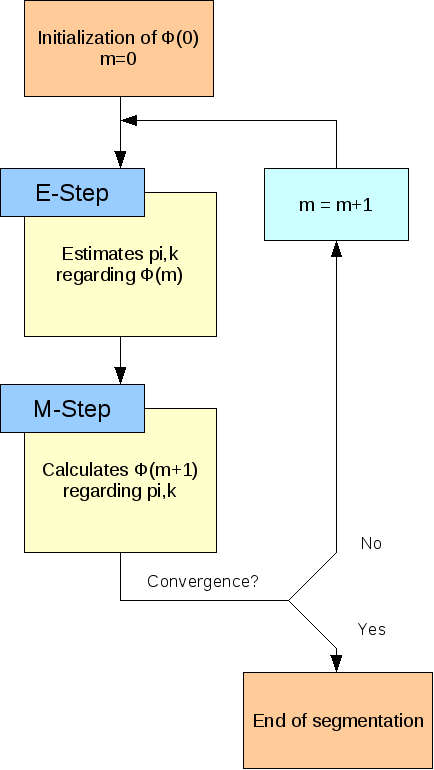
\includegraphics[width=.4\textwidth]{Images/Graphics/EMSimple.png}
  \caption{Basic EM algorithm}\label{fig:EMAlgorithm}
  \end{figure}

\section{Expectation maximization algorithm used in Slicer 3}\label{angels}
In this part, we present the EM algorithm which has been intergated in Slicer 3 and the worklow in which it ahs been integrated as well. Finally, we briefly discuss of the limitations of this one.
\par
The EM algorithm which is used in the SPL is a derived one, from the original one. It enhances the original algorithm adding informations like a probalistic atlas, a multichannel segmentation, a bias correction and a structure information. In Slicer 3, the GMM is used to describe the tissues to segment. Thus it will simplify the problem and the notations.
%
\subsection{Probabilistic atlas}\label{spatial}
The EM algorithm is very sensitive to initialization since it only finds local extremums during the maximization step. A solution to enhance the initialization is to use atlases. There is an atlas for each class you want to segment. For each voxel $i$ of the volume, it returns the probability that this voxel belongs to class $k$. This probability can be used as initialization.
  \begin{equation*}
  p_{ik}^{(0)} = p_{ik}^{atlas}
  \end{equation*}   

From this value, it estimates $\Phi^{(1)}$ and the algorithm iterates until convergence is reached. The probabilistic atlases are not only used to inialize the process. It is also use to get a more robust algorithm. Indeed, we can use the spatial information given by the atlases. Voxels will be classified not only based on intensity but regarding spatial position as well. Van Lemput \textit{et al.} (\cite{8} and \cite{9}) used the spatial prior at each iteration. It is constant and we then have a spatial information. The probability that a pixel $i$ belongs to class $k$, in the E-Step changes. From equation ~(\ref{ESTEP1}), it becomes:

  \begin{equation*}\label{ESTEP2}
  p_{ik}^{(m+1)} = \frac{p(Y_i|e_k,\Phi^{(m)}p_{ik}^{atlas}}{\sum_{j=1}^K   p(Y_i|e_j,\Phi^{(m)}) p_{ik}^{atlas}}  
  \end{equation*}

%
\subsection{Multichannel segmentation}\label{multichannel}
Most of the time, several modalities are used to process brain segmentation. Indeed, the best suited modality to use depends on the tissue you want to segment. For example, T1\footnote{MR images acquisition sequence designed to enhance the grey matter/white matter contrast. See \cite{12}.} MR images are well suited to segment white matter (WM) but are really bad for cerebrospnial fluid (CSF). On the contrary, T2\footnote{MR images acquisition sequence designed to enhance the grey matter/cerebrospinal fluid contrast. See \cite{12}.} MR images are well suited for CSF and not for WM. To formalize the utilisation of different MR images sequences during the segmentation, we will change the definition of $y_i$ and of $\mu_k$ we did at the beginning.Let $y_i = \{y_{i1},y_{i2}, ..., y_{iR}\}$ and $\mu_i = \{\mu_{i1},\mu_{i2}, ..., \mu_{iR}\}$ when we use $R$ images, from different modalities to do the segmentation. The equations for the E-Step and the M-Step will remain the same.
%
\subsection{Bias field correction}\label{biasfield}
A major issue in MR modality is that the images can be corrupted by a low field bias field. It is due to equipment limitations or/and to patient induced electrodynimic interactions (\cite{12}). We will now present how this bias field can be estimated and corrected in the EM algorithm.
%
\subsubsection{Principle}
Let $I=(I_1, ..., I_n)$ the observed intensities in an image, $I^*=(I_1^*, ..., I_n^*)$ the ideal intensities and $F=(F_1, ..., F_n)$ the bias field. Then, the degradation at each voxel can be expressed as:

  \begin{equation*}
  I_i=I_i^*F_i
  \end{equation*}

Let $Y=(Y_1, ..., Y_n)$ and $Y^*=(Y_1^*, ..., Y_n^*)$ be the log-transformed observed and ideal intensities.$B=(B_1, ..., B_n)$ the log-bias field. This transforms makes the bias field becomes additive instead of multiplicative without the log-approach.

  \begin{equation*}
  Y_i=Y_i^* + B_i
  \end{equation*}
  
We can model the PDF of the voxel intensity with a gaussian distribution

 \begin{equation*}
  p(y_i|e_k, \Phi, B) = G(y_i-b_i,\mu_k,\sigma_k)
  \end{equation*}
  
The low frequency characteristic of the bias field $B$ can be modeled by a linear combination of smooth basics functions $\Psi_l(x)$ (\cite{13}). Let $b_i$ be the realisation of the random variable $B_i$ 

  \begin{equation*}
  b_i = \sum_{l=1}^L a_l\Psi_l(pos(i))
  \end{equation*}
  
 $pos(i)$ returns the 3D position $(x,y,z)$ of the voxel $i$. $a_i$ is the $i^{(th)}$ value of the vector $A=(a_1, ..., a_L)$. $A$ represents the bias field parameters.
 \par
In the GM model, bias field can then be estimated using EM framework. The bias field parameter $A$ will be used during the E-Step , through $bi$ to estimate the soft segmentation. $A$ will be re-estimated during the M-Step, after the maximization of the tissue class parameters (mean, variance and weight).
Van Leemput formalised the two steps as below (\cite{8} and \cite{9}):\\

%\par
\begin{itemize}

\item\textbf{E-step}\\
  \begin{equation*}
  p_{ik}^{(m+1)}= \frac{G(y_i-b_i,\mu_k^{(m)},\sigma_k^{(m)})p_{ik}^{atlas}}{\sum_{j=1}^K G(y_i-b_i,\mu_j^{(m)},\sigma_j^{(m)})p_{ij}^{atlas}}\\
  \end{equation*}
  
%\par
\item\textbf{M-step}\\
  \begin{itemize}

  \item Gaussian distribution parameters estimation
    
    \begin{equation*}
    \mu_k^{(m+1)} = \frac{\sum_{i=1}^n y_ip_{ik}^{(m+1)}-b_i}{\sum_{i=1}^n p_{ik}^{(m+1)}}\\
    \end{equation*}

    \begin{equation*}
    (\sigma_k^{(m+1)})^2 = \frac{\sum_{i=1}^n (y_i-\mu_k^{(m+1)}-b_i)^2p_{ik}^{(m+1)}}{\sum_{i=1}^n p_{ik}^{(m+1)}}\\
    \end{equation*}

  \item Bias field correction

  \begin{equation}\label{BIASFIELD}  
  (A^{(m+1)})^T = (F^TW^{(m+1)}F)^{-1}F^TW^{(m+1)}R^{(m+1)}  
  \end{equation}

with:

  \begin{equation*}
   \mathbf{F} = \left(
  \begin{array}{clcr}
   \Psi_1(pos(1)) & \Psi_2(pos(1)) & \ldots & \Psi_L(pos(1)) \\
   \Psi_1(pos(2)) & \Psi_2(pos(2)) & \ldots & \Psi_L(pos(2)) \\
   \vdots & \vdots & \ddots \\
   \Psi_1(pos(N)) & \Psi_2(pos(N)) & \ldots & \Psi_L(pos(N)) \\
  \end{array} \right)
  \end{equation*}
  
  \begin{equation*}
   \mathbf{W^{(m+1)}} = \left(
  \begin{array}{clcr}
   \sum_{k=1}^K w_{1k}^{(m+1)} & 0 & \ldots & 0 \\
   0 & \sum_{k=1}^K w_{2k}^{(m+1)} & \ldots & 0 \\
   \vdots & \vdots & \ddots \\
   0 &  \ldots & 0 & \sum_{k=1}^K w_{Nk}^{(m+1)} \\
  \end{array} \right)
  \end{equation*}

  \begin{equation*}
  w_{ik}^{(m+1)}  = \frac{p_{ik}^{(m+1)}}{(\sigma_k^{(m+1)})^2}\\
  \end{equation*}
  
  \begin{equation*}
   \mathbf{R} = \left(
  \begin{array}{cl}
   y_1 - \tilde{y}_1^{(m+1)} \\
   \vdots\\
   y_N - \tilde{y}_N^{(m+1)} \\
  \end{array} \right)
  \end{equation*}
  
  \begin{equation*}
  \tilde{y}_i^{(m+1)}  = \frac{\sum_{k=1}^K w_{ik}^{(m+1)} \mu_{ik}^{(m+1)}}{\sum_{k=1}^K w_{ik}^{(m+1)}}
  \end{equation*}


  \end{itemize}

\end{itemize}

The bias field correction can be interpreted as follows: the estimated soft segmentation ($p_{ik}^{(m)}$) and tissue class parameters are used to reconstruct the image $\tilde{Y}=(\tilde{y_1}, ..., \tilde{y_n})$. This new image is supposed not to be corrupted by the bias field. We then substract the reconstructed image $\tilde{Y}$ from the observed image $Y$. We obtain the residual image $R$. From $R$, we estimate the bias field. $F$ represents the discretized geometry of the bias field. $W$ is an inverse covariance matrix. It returns informations about the possible error for each voxel. The covariance matrix will be descibed in details in section (QSDQSD).
\par
The approach used in Slicer 3 is based on the same principle but differs regarding the maximization method and the parameter which is maximized.
%
\subsubsection{Variation used in Slicer 3}
In this method, we are working with a GMM. Moreover the parametres of this gaussian distribution are assumed to be known. The idea of estimating the field in EM framework was originally proposed by Wells \textit{et al.} (\cite{10}). He proposed to only use maximization to re-estimate the bias field. The \textit{maximum a posteriori principle} (MAP) instead of the maximum likelihood principle (equation (~\ref{AR})) is used to find the lower bound, duringthe maaximization:

\begin{align*}\label{ARMAP}
  \hat{\Phi} &=\operatorname*{arg\,max}_\Phi p(\Phi |Y)\\
             &\mbox{As Bayes's theorem can be applied} \\
             %&{now we remove the terms which are constants regarding \Phi }\\
             &=\operatorname*{arg\,max}_\Phi \frac{p(Y|\Phi)p(\Phi)}{p{Y}}\\  
             &\mbox{As $p(Y)$ do not depend on $\Phi$} \\
             &=\operatorname*{arg\,max}_\Phi p(Y|\Phi)p(\Phi)\\
             %&{now we remove the terms which are constants regarding \Phi }\\
  \end{align*}

Proceeding the same way as we did in section~\ref{GENERAL}, the new E-Step becomes:

\begin{equation}\label{EMAP}
E_{MAP} = E_{Z|Y,\Phi^{(m)}}\{ \operatorname*{ln} p(Y,Z|\Phi) \} + \operatorname*{ln} p(\Phi)
\end{equation}

In Wells' method, the only parameter to be estimate is the bias field. We assume that the noise has a gaussian distribution:

  \begin{equation*}
  p(\Phi) = p(B) = G(B,0,\Sigma_B)
  \end{equation*}
  
The equation for the bias field will change. We add the smoothness constraint in the gaussian distribution: $\Sigma_B^{-1}$. We also set $F$ to unix matrix as no parametric model for the bias field is assumed. Finally, we define the mean residual image $\bar{M}^{(m+1)}$

  \begin{equation*}
  \bar{M}^{(m+1)} = W^{(m+1)}R^{(m+1)}
  \end{equation*}

The equation (~\ref{BIASFIELD}) for the bias field will then be remplaced by $(B^{(m+1)})^T$:

  \begin{equation*}
  (B^{(m+1)})^T = (W^{(m+1) + \Sigma_B^{-1}})^{-1}\bar{M}^{(m+1)}
  \end{equation*}

%
\subsection{Hierarchical information}\label{Structure}
The last modification of the original EM algorithm is the addition of hierarchical information in the iterative segmentation process. The algorithm was described by Pohl \textit{et al.} (\cite{11}) The idea was to describe the structures we want to segment as a tree. It allows us to subdivise the segmentation process into subproblems, that are easier to solve, according to Pohl.
  
 % \begin{center}
  \begin{figure}[ht]\centering
  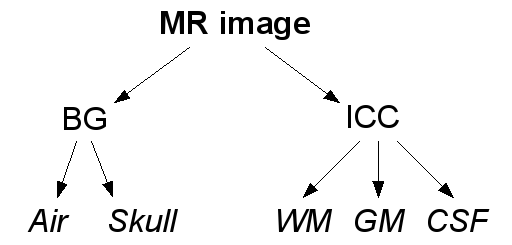
\includegraphics[width=.4\textwidth]{Images/Graphics/treeStructure.png}
  \caption{A simple tree structure of the brain}\label{fig:treeStructure}
  \end{figure}
  
Here we continue with an intuitive description of the process. It is a brief explanation of how the tree figure (\ref{fig:treeStructure}) would be segmented using the tree structure information. At the first iteration, the MR image will be segmented into the background (BG) and the intracranial cavity (ICC) with the EM algorithm. At the second iteration, the BG will be segmented into the air and the skull. Finally, at the last iteration, the ICC will be segmented into white matter (WM), grey matter (GM) and cerebrospinal fluid (CSF).

To formalize it, we incorporate $H$, a set of structure-specific information in equation (\ref{EMAP}). $H$ contains a lot of information like the structures of the tree which have to be segmented, an approximative size of the structure to be segmented and information about which modality is the best suited to segment this structure.
\begin{equation*}
 \Phi^{(m+1)}=\operatorname*{arg\,max}_\Phi \{\sum_{k=1}^K   (p(e_{k}|Y,\Phi^{(m)},H)\operatorname*{log} p(Y,e_{k}|\Phi,H)) + \operatorname*{ln} p(\Phi ,H) \} \\
\end{equation*}
%  \end{center}
 
\subsection{Summary}\label{SUMMARY}
We have shown that the EM algorithm is very flexible and can be transformed to solve a lot of segmentation problems. It is very well suited for segmentation of MR brain images and we can add a lot of informations through this algorithm to enhance the segmentation. The iterative general process is divided in two steps: the expectation (E-Step) and the maximization (the M-Step).

  \begin{itemize}
  \item \textbf{E-Step}\\  
  Estimates a soft segmentation ($p_{ik}$), given parameter $\Phi^{(m)}$. The soft segmentation creates a map of probability. Each voxels contains the probabilities that it belongs to each class. It is used for the final segmentation.
  
  \item \textbf{M-Step}\\
  Estimates $\Phi^{(m+1)}$, using the soft segmentation done in the E-Step.
  
    \begin{itemize}
    \item Estimates the intensity distribution for each intensity class.    
    \item Estimates the bias field, $\Phi^{(m+1)}$, using the soft segmentation and the intensity class distribution
    \end{itemize}
  \end{itemize}
  
Each node will then be segmented until the whole tree has been processed as described in section (\ref{Structure}).

  \begin{figure}[ht]\centering
  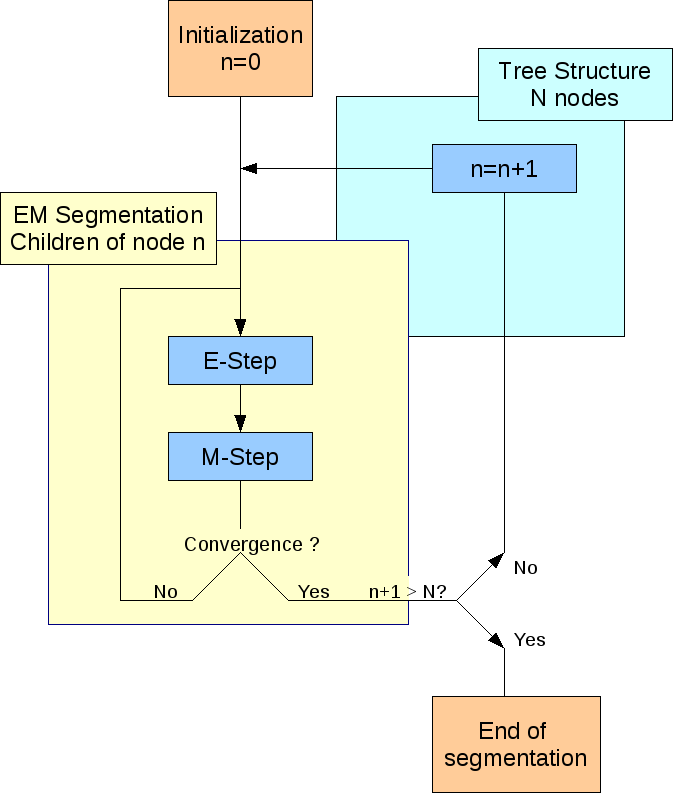
\includegraphics[width=.6\textwidth]{Images/Graphics/workflowtheorical.png}
  \caption{EM segment algorithm in Slicer}\label{fig:EMSSlicer}
  \end{figure}
  
We can also describe the segmentation process in the figure (\ref{fig:EMSSlicer}). To describe how it works, we use the tree structure presented in figure (\ref{fig:treeStructure}) . It first segments the node $n=0$, i.e., BG and ICC. Once the EM Segmentation has converged, BG and ICC have been segmented and we move to the next node. Air and Skull will then be segmented. Following this process, all the structures of the tree will be segmented.
%
\section{Workflow in Slicer 3}
We will now present the whole segmentation framework used in Slicer 3. This will describe all the initialisation steps done by the user, via the graphical user interface (GUI). It will also present how the whole algorithm works. We will remind why is each initialisation step important and where is this information used.
%
\subsection{User interface}\label{GUI}
It consists in a manual initialization of the parameters which are require for the segmentation on Slicer 3. The user chooses the good values via the GUI.

\begin{itemize}
\item \textbf{Step 1: Tree structure creation}\\
\hspace*{4 mm}We first create the tree structure we want to use for the segmentation. It will be used to define $H$ (section (\ref{Structure})).
%
\item \textbf{Step 2: Atlas assignment}\\
\hspace*{4 mm}We assign to each node of the tree, i.e. to each tissue to segment, the related atlas. It will be used for the spatial information (section (\ref{spatial})). It implies that you need an atlas for each structure that you want to segment.
%
\item \textbf{Step 3: Multimodal segmentation}\\
\hspace*{4 mm}We choose the images we want to use for the segmentation. As discussed in section (\ref{multichannel}), it is usefull for the mutlichannel segmentation since some tissues are not clearly visible in some modalities.
%
\item \textbf{Step 4: Intensity normalization}\\
\hspace*{4 mm}We choose the value for the intensity normalization. We normalize the intensity of the images to be segmented, regarding the atlas. The target images are normalized. Thus, they have the same mean intensity as the related atlas. It is usefull if we want to use the command-line module. Doing an intensity normalisation, the initialisation value of each class will be the same for each volume. It is a convenient way to run a lot of segmentation.
%
\item \textbf{Step 5: Class definition}\\
\hspace*{4 mm}We define mean value, variance and covariance for each class and modality. Moreover, it is precise way to initialiase the class tissues distribution for the algorithm. It it usefull because the EM algorithm used only estimates the bias field but still requires informations about the tissues to be segmented. Using these values, the algorithm is can be initialized then estimates the bias.
%
\item \textbf{Step 6: Prior weights}\\
\hspace*{4 mm}We define the importance of each target image and of the atlas for each tissue to segment. It is will be usefull to define $H$ (section ~\ref{Structure}). For each tissue, $H$ knows usefull informations like which modality is the more relevant  for the class and the size that the class is supposed to be.
\par
\hspace*{4 mm}For example, for the CSF. Let's assume that we proceed to a multi channel segmentation with T1 and T2 MR images. We give a weight of one (maximum) to the T2 target volume and zero (minimum) to the T1 target volume. It means that the only relevant information for CSF will be in the T2 volume. The algorithm will act in consequence and only use the information from T2 to do the segmentation. It is the same for the atlas. If we set the weight of the atlas to one, the algorithm will use the spatial information. If we set it to zero, it will not.
%
\item \textbf{Step 7: Registration method}\\
\hspace*{4 mm}We choose the type of registration we want. Different kind of registrations are available. The default registration method is a non-rigid registration. The point of choising a registration method is presented in the next section.
\end{itemize}
%
\subsection{Algorithm}
After all the initialisation steps done via the GUI (section ~\ref{GUI}), we will no present the core of the segmentation pipeline.
%
\begin{itemize}
\item \textbf{Step 1: Intensity normalisation}\\
\hspace*{4 mm}The intensity of the target volumes are normalized to the value that the user chose in the GUI. The utility of this treatment has been discissed in the previous section, at the step 4.
%
\item \textbf{Step 2: Images registration}\\
\hspace*{4 mm}In order for the atlas to guide the segmentation (spatial information), it as to be aligned to the target images. The transformation is evaluated between the first normalized target image and its atlas.
%
\item \textbf{Step 3: Spatial prior alignement}\\
\hspace*{4 mm}The transformation computed during the image registration is applied to all the structure-specific atlases. 
%
\item \textbf{Step 4: EM Algorithm in the tree structure}\\
\hspace*{4 mm}The whole segment workflow is then applied (section~\ref{SUMMARY}).

\end{itemize}
%
\subsection{Summary}
In Slicer 3, the whole segmentation pipeline can be described as in figure (\ref{fig:Wpipeline}). There is first an iniatialization step, done by user via the GUI. Then, some pre-processing steps are applied in order to enhance the segmentation. Finally, the EM algorithm segments the MR images.

  \begin{figure}[ht]\centering
  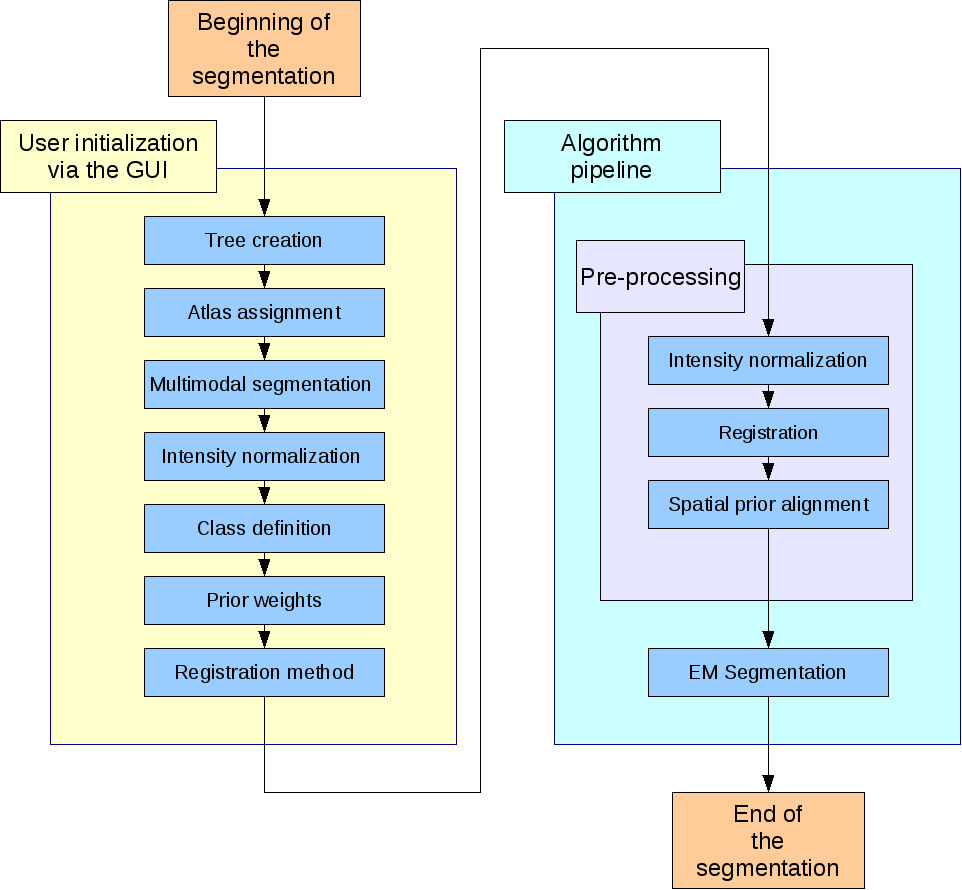
\includegraphics[width=0.8\textwidth]{Images/Graphics/wholepipeline.png}
  \caption{The whole segmentation pipeline in Slicer 3}\label{fig:Wpipeline}
  \end{figure}

%
\section{Limitations}\label{su:limitations}
Even if the EM segmentation pipeline is robust in Slicer 3, some limitations appear.
\par
The first problem the user has to face appears during the intensity normalization step. The user has no tools to find the good normalization value. He has to guess it. This problem will be discussed in section SDFSDF.
\par
The second problem is directly linked to the EM algorithm. As the maximization method is a local one, the class distribution, which are used for the initialization of the algorithm have to be well defined. So far, we have no possibilities to know how accurate our definition of the class is. This problem will be discussed in details in section SDFSDF.
\par
Another problem appears at the same steps. The actual method for defining means and variances for each class appears not as efficient as we want it to be. This problem will be discussed in details in section SDFSDF.
\par 
The last problem we encountered appeared after the initialization, during the pre-processings. Only one pre-processing (intensity normalization) is done on the target images before the registration to the atlas. Since the EM algorithm is mainly designed to work on MR images, bias field is a recurrent problem. Proceeding to a registration before a bias correction can deteriore a lot the results of the registration. This problem will be discussed in details in section SDFSDF.\\

%
\par
After this presentation of the main issues, we will in the next chapter explain the problems more deeply and show you the solutions we brought to solve it.
